\section{Métodos de divisor}

%"The decisive conclusion of the preceding section is that the
%only realistic candidates for methods of apportionment are the divisor methods. 
%The question then becomes: which of the infinite number of divisor 
%methods should be chosen?" \cita{balinski1980theory}
%
%"Divisor methods fix the rounding rule and adjust the divisor. Quota
%methods fix the divisor and adjust the rounding rule." \cita{pukelsheim2017}

Parte fundamental de la esencia del problema de apportionment radica en la dificultad de 
definir cómo redondear satisfactoriamente las partes fraccionarias de las quotas: el método de
Webster, por ejemplo, divide los votos de cada partido por un divisor $d$ y luego redondea los resultados utilizando el método 
tradicional de redondeo al entero más cercano. Por su parte, el método D'Hondt utiliza la función "piso",
redondeando a la parte entera. Para extender esta metodología y poder considerar otros métodos necesitamos
introducir las nociones de "función de redondeo" y "regla de redondeo", que nos permitirán definir la familia de 
métodos de divisor.

\begin{definition}
    (\textbf{Función de redondeo})
    Una función de redondeo se define como una función 
    \[
    f: [0,\infty) \rightarrow \mathbb{N}_0 \ \text{creciente y sobreyectiva.}
    \]
\end{definition}

El hecho de que una función de redondeo sea creciente y sobreyectiva implica que 

$$f(0) = 0,$$

y que 

\begin{align*}
[0,\infty) 
&= \bigcup\limits_{i \in \mathbb{N}_0} f^{-1}(\{ i \}) \\
&= \bigcup\limits_{i \in \mathbb{N}_0} [s_i, s_{i+1}),
\end{align*}

para $s_i \vcentcolon= \min \{s \in \mathbb{R}_{\geq 0} : f(s) = i\}$, por lo que podemos pensar 
en una función de redondeo $f$ a partir de la sucesión $(s_i)_{i \in \mathbb{N}_0}$. 
A esta sucesión la denominamos \textit{secuencia de saltos}.
Esta caracterización establece que $f(s_i) = i \ \forall i \in \mathbb{N}_0$. Pensando en el redondeo de $j + \frac{1}{2}$ para 
$j \in \mathbb{N}_0$, no es claro que siempre vayamos a querer que sea redondeado hacia abajo, por lo que podríamos incluir la posibilidad de que 
$f(j + \frac{1}{2}) = \{j, j + 1\}$ para tener una noción un poco más general. Para los puntos de 
la \textit{secuencia de saltos}, esto se traduciría en definir $f(s_j) = \{j-1, j\}$. Detallamos esta idea en la definición
de "regla de redondeo":

\begin{definition}
(\textbf{Regla de redondeo})
Una regla de redondeo $\llbracket \cdot \rrbracket$ dada por una \textit{secuencia de saltos}
$0 = s(0) \leq s(1) < s(2) < \dots$ se define como

\[
    \llbracket t \rrbracket = 
    \begin{cases}
        \{ 0 \}, & \text{si } t=0 \\[6pt]
        \{ n \}, & \text{si } t \in (s(n), s(n+1)) \\[6pt]
        \{ n-1, n \}, & \text{si } t = s(n)
    \end{cases}
\]
    
\end{definition}


Esta definición nos permite identificar de manera unívoca cualquier regla de redondeo a partir de su secuencia de saltos subyacente, 
por lo que utilizaremos cualquiera de estas dos caracterizaciones de manera indistina. La relación fundamental que nos permite entender 
mejor el vínculo es la siguiente:

\[
n \in \llbracket t \rrbracket \text{ si y solo si } s(n) \leq t \leq s(n+1) \quad \forall n \in \mathbb{N}, t \geq 0.
\]

\vspace{1em}

En principio, partiendo de la definición anterior, una secuencia de saltos podría tener varios puntos concentrados 
en un mismo intervalo de la forma $[n, n+1]$ para $n \in \mathbb{N}$, como podemos observar en el siguiente ejemplo:


\begin{figure}[h!]
\centering
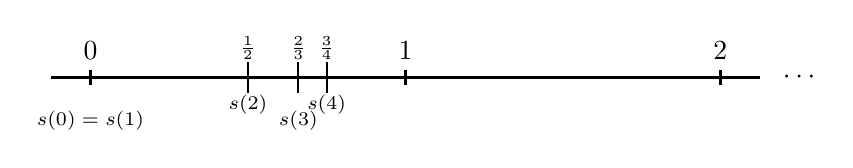
\begin{tikzpicture}[scale=1, baseline={(0,0)}]
    % Eje principal
    \draw[thick] (-0.5,0) -- (8.5,0);

    % Marcas principales
    \foreach \x in {0,4,8}
        \draw[very thick] (\x,0.1) -- (\x,-0.1);
    \foreach \x in {2,2.64,3}
        \draw[thick] (\x,0.2) -- (\x,-0.2);

    % Etiquetas superiores
    \node[above] at (0,0.1) {$0$};
    \node[above] at (4,0.1) {$1$};
    \node[above] at (8,0.1) {$2$};
    \node[above] at (2,0.1) {\scriptsize $\frac{1}{2}$};
    \node[above] at (2.64,0.1) {\scriptsize $\frac{2}{3}$};
    \node[above] at (3,0.1) {\scriptsize $\frac{3}{4}$};

    % Etiquetas inferiores
    \node[below] at (0,-0.3) {\scriptsize $s(0)=s(1)$};
    \node[below] at (2,-0.1) {\scriptsize $s(2)$};
    \node[below] at (2.64,-0.3) {\scriptsize $s(3)$};
    \node[below] at (3,-0.1) {\scriptsize $s(4)$};

    % Puntos suspensivos
    \node at (9,0) {$\cdots$};
\end{tikzpicture}
\caption{Ejemplo de secuencia de saltos espuria, con $s(0) = 0; s(i) = 1 - \frac{1}{i} \quad \forall i \in \mathbb{N}$.}
\label{fig:sucesion-espuria-s}
\end{figure}

\vspace{1em}

Como queremos evitar esto, extenderemos la definición de \textit{secuencia de saltos} para que solamente contemple sucesiones
"razonables". Este término lo entendemos en el sentido de que los números redondeados a $n \in \mathbb{N}$ deben tener a $n$ cerca, es decir, 
$n \in [s(n), s(n+1)]$.

\begin{definition}
    (\textbf{Secuencia de saltos})
    Llamamos \textit{secuencia de saltos} a una sucesión $(s(0), s(1), s(2), \dots)$ que verifica las siguientes propiedades:
    \begin{enumerate}[label=\roman*)]
        \item (\textit{Inicialización}) $s(0) = 0$;
        \item (\textit{Localización}) $s(n) \in [n-1, n] \quad \forall n \in \mathbb{N}$;
        \item (\textit{Disjunción izq-der})
            $$s(n) = n-1 \text{ para algún } n \in \mathbb{N} \implies s(m) < m \ \forall m \in \mathbb{N}$$
            $$s(n) = n \text{ para algún } n \in \mathbb{N} \implies s(m) < m-1 \ \forall m \in \mathbb{N}$$
    \end{enumerate}
\end{definition}

Esta última condición nos permite concluir que, exceptuando $s(1)$ -- cuyo valor podría ser $0 = s(0)$ --, la secuencia
será estrictamente creciente. Para ver esto, basta observar que la única forma de que dos términos consecutivos coincidan
es si $s(n) = n = s(n+1)$ para algún $n \in \mathbb{N}$. Esta posibilidad queda excluida por la condición $\text{\small III)}$ de 
\textit{Disjunción izq-der}, puesto que $s(n) = n \implies s(m) > m \ \forall m \in \mathbb{N}$, y de forma análoga se ve el otro caso.

Con esta nueva definición de \textit{secuencia de saltos} podemos descomponer al intervalo $[0; +\infty)$ como 

\[
    \bigcup\limits_{i \in \mathbb{N}_0} [s(i), s(i+1)),
\]

pero ahora con la garantía de que $n \in [s(n), s(n+1)]$.

\vspace{2em}

\begin{example}
    (\textbf{Secuencias de saltos estacionarias})
    Un caso particular -- y bastante natural de definir-- de secuencias de saltos son las \textit{secuencias de saltos
    estacionarias}, que dependen de un parámetro $r \in [0;1]$ y se definen como
    \begin{align*}
        s_r(0) &= 0; \\
        s_r(n) &= n - 1 + r \quad \forall n \in \mathbb{N};
    \end{align*}
    por lo que dividen al intervalo real no negativo en los puntos $0, r, 1+r, 2+r, \dots$.

    Esta familia de métodos recorre un amplio espectro de reglas de redondeo típicas:
    para $r=0$ define el método de redondeo usualmente denominado \textit{"techo"} o \textit{"redondeo hacia arriba"} y denotado $\lceil \cdot \rceil$;
    para $r=\frac{1}{2}$ define el método de redondeo tradicional;
    para $r=1$ define el método de redondeo usualmente denominado \textit{"piso"}, \textit{"redondeo hacia abajo"} o \textit{"parte entera"}, denotado $\lfloor \cdot \rfloor$.
\end{example}

\begin{figure}[h!]
\centering
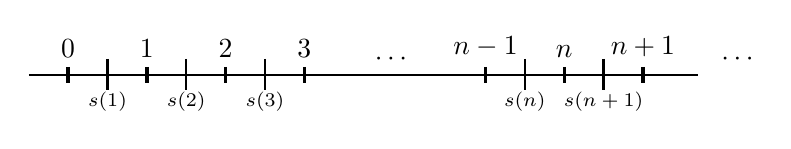
\begin{tikzpicture}[scale=1, baseline={(0,0)}]
  % Eje principal
  \draw[thick] (-0.5,0) -- (8,0);

  % Marcas principales
  \foreach \x in {0,1,2,3}
    \draw[very thick] (\x,0.1) -- (\x,-0.1);
  \foreach \x in {0.5,1.5,2.5}
    \draw[thick] (\x,0.2) -- (\x,-0.2);

  % Etiquetas superiores
  \node[above] at (0,0.1) {$0$};
  \node[above] at (1,0.1) {$1$};
  \node[above] at (2,0.1) {$2$};
  \node[above] at (3,0.1) {$3$};

  % Etiquetas inferiores
  \node[below] at (0.5,-0.1) {\scriptsize $s(1)$};
  \node[below] at (1.5,-0.1) {\scriptsize $s(2)$};
  \node[below] at (2.5,-0.1) {\scriptsize $s(3)$};

  % Puntos suspensivos
  \node at (4.1,0.2) {$\cdots$};

  % Últimas marcas
  \draw[very thick] (5.3,0.1) -- (5.3,-0.1);
  \draw[very thick] (6.3,0.1) -- (6.3,-0.1);
  \draw[very thick] (7.3,0.1) -- (7.3,-0.1);
  \foreach \x in {5.8,6.8}
    \draw[thick] (\x,0.2) -- (\x,-0.2);

  % Etiquetas superiores (últimas)
  \node[above] at (5.3,0.1) {$n-1$};
  \node[above] at (6.3,0.1) {$n$};
  \node[above] at (7.3,0.1) {$n+1$};

  % Etiquetas inferiores (últimas)
  \node[below] at (5.8,-0.1) {\scriptsize $s(n)$};
  \node[below] at (6.8,-0.1) {\scriptsize $s(n+1)$};

  % Puntos suspensivos al final
  \node at (8.5,0.2) {$\cdots$};
\end{tikzpicture}
\caption{Ejemplo de secuencia de saltos estacionaria con $r=\frac{1}{2}$: $s_{r}(i) = i - \frac{1}{2}$.}
\label{fig:sucesion-s}
\end{figure}

Quizás pueda parecer inútil definir reglas de redondeo de esta forma tan general, pero basta observar el siguiente ejemplo
para darse cuenta de que los métodos más típicos ($\lceil \cdot \rceil$, $\lfloor \cdot \rfloor$, redondeo estándar) no permiten
resolver de forma satisfactoria ciertos escenarios.

\begin{table}[h!]
\centering
\begin{tabular}{lrrr}
\hline
\textbf{1975} & \textbf{Población} & \textbf{Proporción} & \textbf{Porcentaje} \\
\hline
Asia                  & 2\,295\,000\,000 & 0.57289 & 57 \\
Europa                &   734\,000\,000 & 0.18323 & 18 \\
Américas              &   540\,000\,000 & 0.13480 & 13 \\
África                &   417\,000\,000 & 0.10409 & 10 \\
Australia y Oceanía   &    20\,000\,000 & 0.00499 &  0 \\
\hline
\textbf{Suma}         & 4\,006\,000\,000 & 1.00000 & 98 \\
\hline
\end{tabular}
\caption{\small Porcentajes de población por continente de acuerdo a la regla estándar de redondeo.
Se observa cómo esta regla de redondeo no basta para alcanzar una solución en la que la suma de porcentajes sea efectivamente del $100\%$.
Tabla extraída de \cita{pukelsheim2017}}
\end{table}


\begin{definition}
    \textbf{(Métodos de divisor)}
    Consideramos como método de divisor inducido por la regla de redondeo $\llbracket \cdot \rrbracket$ a aquél método de \textit{apportionment} 
    cuya imagen es el conjunto de asignaciones dado por
    \[
        A(\vec{v}, H) \vcentcolon= \left\{ (x_1, \dots, x_n) \in \mathbb{N}^{n}(H) : x_i \in \Big\llbracket \frac{v_i}{D} \Big\rrbracket 
        \ \forall i \in [n], \text{ para cierto } D > 0 \right\}.
    \]
\end{definition}

\vspace{2em}
La idea de esta familia de métodos es "dividir y redondear" (\cite{pukelsheim2017}), dividiendo los votos por cierto divisor 
$D>0$ y luego aplicando la regla de redondeo $\llbracket \cdot \rrbracket$ a los resultados, de forma tal que tomando 
cantidades $x_i \in \Big\llbracket \frac{v_i}{D} \Big\rrbracket$, los vectores resultantes sean asignaciones válidas, ie
$x_+ = H$.


\begin{proposition}
    Los métodos de divisor satisfacen anonimidad, balance, concordancia, decencia y exactitud.
    \begin{proof}
        La demostración no es ni muy relevante ni muy instructiva, por lo que no la realizaremos en el presente trabajo.
    \end{proof}
\end{proposition}


\begin{theorem}
    (\textbf{Desigualdad max-min})
    
    Sea $A$ el método de divisor inducido por la regla de redondeo con secuencia de saltos $s(0), s(1), s(2), \dots$.
    
    Entonces, una asignación de bancas $x \in \mathbb{N}^{n}(H)$ pertenece al conjunto de asignaciones de bancas para el vector $\vec{v} \in (0, \infty)^n$
    dado por $A(\vec{v}, H)$ si y solo si

    \begin{align*}
        \max\limits_{j \in [n]} \frac{v_j}{s(x_j + 1)} \leq \min\limits_{j \in [n]} \frac{v_j}{s(x_j)}
    \end{align*}

    Esta desigualdad nos brinda el rango de valores en el que podemos tomar el divisor $D > 0$ tal que $x \in A(\vec{v}, H)$.
    
    \begin{proof}
        $x$ es una asignación dada por el método de divisor $A$ si y solo si $\exists D > 0$ tal que 
        $x_j \in \llbracket \frac{v_j}{D} \rrbracket \ \forall j \in [n]$, lo cual sucede si y solo si
        \begin{align*}
            s(x_j) \leq \frac{v_j}{D} \leq s(x_j + 1) \ \forall j \in [n] \ &\iff \\
            \frac{v_j}{s(x_j + 1)} \leq D \leq \frac{v_j}{s(x_j)}  \ \forall j \in [n] \ &\iff \\
            \max\limits_{j \in [n]} \frac{v_j}{s(x_j + 1)} \leq D \leq \min\limits_{j \in [n]} \frac{v_j}{s(x_j)} &\implies \\
            \max\limits_{j \in [n]} \frac{v_j}{s(x_j + 1)} \leq \min\limits_{j \in [n]} \frac{v_j}{s(x_j)}
        \end{align*}
        Y esto demuestra la ida. 

        Para la vuelta, el hecho de que se verifique la desigualdad max-min garantiza la existencia de $D > 0$ para que $x \in A(\vec{v}, H)$.
    \end{proof}
\end{theorem}

Definiremos los siguientes conjuntos de índices, que permitirán entender cómo construir nuevas soluciones a partir de una solución
dada:

\begin{align*}
    I(x, v) = \left\{ i \in [n] : \frac{v_i}{s(x_i + 1)} = \max\limits_{j \in [n]} \frac{v_j}{s(x_j + 1)} \right\} \\
    K(x, v) = \left\{ k \in [n] : \frac{v_k}{s(x_k)} = \min\limits_{j \in [n]} \frac{v_j}{s(x_j)} \right\} \\
\end{align*}

\begin{proposition}
    (\textbf{Unicidad de divisor})

    Dados $A$ un método de divisor, $H \in \mathbb{N}$ y $\vec{v} \in \mathbb{R}_{\geq 0}^n$, se tiene que

    $$\{ x \} = A(\vec{v}, H) \iff \max\limits_{j \in [n]} \frac{v_j}{s(x_j + 1)} < \min\limits_{j \in [n]} \frac{v_j}{s(x_j)}$$
    $$\{ x \} \subsetneq A(\vec{v}, H) \iff \max\limits_{j \in [n]} \frac{v_j}{s(x_j + 1)} = \min\limits_{j \in [n]} \frac{v_j}{s(x_j)}$$

    Esto nos dice que el divisor $D > 0$ para el cual el método $A$ queda bien definido es único solamente si 
    $A$ retorna soluciones múltiples.

    \begin{proof}
        Teniendo en cuenta que ambas condiciones son complementarias, basta con probar la segunda.
        
        Para la ida, supongamos que $x, y \in A(\vec{v}, H)$ son dos soluciones distintas, $x \neq y$.
        Sean $D(x), D(y)$ divisores para $x$ e $y$ respectivamente. Si se tuviera que
        $D(x) > D(y)$, por monotonía valdría que $x_i \leq y_i \ \forall i \in [n]$. Dado que el total de bancas
        es igual para ambos vectores -- $x_+ = y_+ = H$--, ambos vectores deben coincidir, contradiciendo 
        el hecho de que sean distintos, por lo que no puede suceder que $D(x) > D(y)$. 
        De igual forma se ve que tampoco vale $D(x) < D(y)$, por lo que se concluye que $D(x) = D(y) = D$.
        Se tiene entonces que $x_i, y_i \in \llbracket \frac{v_i}{D} \rrbracket \ \forall i \in [n]$. 
        Como $x \neq y$ y $x_+ = y_+ = H$, debe haber dos componentes $j \neq k$ tales que $x_j < y_j$ y $x_k > y_k$.
        Pero como $x_j, y_j \in \llbracket \frac{v_i}{D}$, debe tenerse $x_j + 1 = y_j$, y se debe cumplir 
        $\frac{v_j}{D} = s(x_j + 1)$. De igual forma, $x_k = y_k + 1$, y se tiene el empate $\frac{v_k}{D} = s(x_k)$.
        En consecuencia,

        $$D = \frac{v_j}{s(x_j + 1)} \leq \max\limits_{i \in [n]} \frac{v_i}{s(x_i + 1)} \leq 
        \min\limits_{i \in [n]} \frac{v_i}{s(x_i)} = \frac{v_k}{s(x_k)} = D,$$

        por lo que vale la igualdad en la desigualdad Max-Min.

        Para la vuelta, supongamos que $\max\limits_{i \in [n]} \frac{v_i}{s(x_i + 1)} = 
        \min\limits_{i \in [n]} \frac{v_i}{s(x_i)} = D$.
        Como las opciones de incremento $i \in I(x, v)$ están empatadas -- $\frac{v_i}{D} = s(x_i + 1)$--,
        se redondean a $\llbracket \frac{v_i}{D} \rrbracket = \{ x_i, x_i + 1\}$. Las opciones de decremento
        $k \in K(x, v)$ también se encuentran empatadas -- $\frac{v_k}{D} = s(x_k)$--, por lo que se redondean
        a $\llbracket \frac{v_k}{D} \rrbracket = \{ x_k - 1, x_k\}$. 

        Estos dos conjuntos son disjuntos: $I(x,v) \cap K(x,v) = \emptyset$. Si no fuese el caso, se tendría 
        $j \in I(x,v) \cap K(x,v)$ tal que $\frac{v_j}{s(x_j + 1)} = D = \frac{v_j}{s(x_j)}$, contradiciendo el 
        hecho de que las secuencias de saltos son estrictamente crecientes.
        Luego, podemos tomar $i \in I(x,v)$ y $k \in K(x, v)$, y definir el vector $y$ como
        $y_i = x_i + 1$, $y_k = x_k - 1$, $y_j = x_j \ \forall j \neq i,k$, construyendo otra solución 
        $y \neq x$, $y \in A(H, \vec{v})$. 
    \end{proof}
\end{proposition}


La desigualdad max-min, con la respectiva elaboración de los conjuntos $I(\vec{v}, H)$ y $D(\vec{v}, H)$, ayuda a pensar en 
el siguiente algoritmo polinomial para construir vectores de asignaciones $x \in A(\vec{v}, H)$:

\vspace{0.5em}

\begin{algorithm}[H]
    \SetAlgoLined
    \KwResult{$x \in A(\vec{v}, H)$ vector de asignaciones}
    Tomando $D \vcentcolon= \frac{v_+}{H}$, definir: \\
    \hspace{2em} x$_j = \llbracket \frac{v_j}{D} \rrbracket$ para cada $j \in [n]$ \\
    \If{x$_+=H$}
       {\Return x}
    \Else{
        \If{x$_+ < k$}
        {elegir $i \in I(x, v)$ y aumentar $x_i$ en una unidad \\
         repetir este paso hasta que que x$_+ = H$}
        \Else{elegir $k \in K(x, v)$ y disminuir $x_k$ en una unidad \\
         repetir este paso hasta que que x$_+ = H$}
    }
    \Return x \\
    \caption{Construcción de vector de asignaciones para métodos de divisor.}
\end{algorithm}